\documentclass[a4paper,12pt]{article}

\usepackage{graphicx}
\usepackage{amsmath}
\usepackage{float}

\begin{document}

\noindent
\begin{minipage}[t]{0.2\textwidth}

\includegraphics[width=2.5cm]{iiitb_logo.png}
\end{minipage}
\hfill
\begin{minipage}[t]{0.7\textwidth}
\raggedleft

{\Large \textbf{Pavithra Kune}}

COMETFWC069

\end{minipage}

\vspace{0.8cm}

\begin{center}
{\Large \textbf{GATE QUESTION Q36}}
\end{center}

\vspace{0.3cm}
\hrule
\vspace{0.5cm}

\begin{figure}[H]
\centering
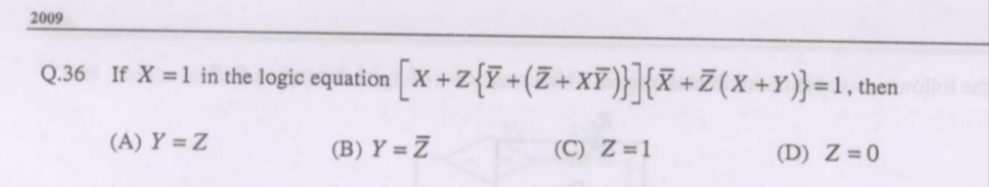
\includegraphics[width=0.8\textwidth]{question.png}
\caption{GATE Question Q36}
\end{figure}

\tableofcontents

\newpage

\section{Components}

Breadboard

Arduino Uno

IC 7447

Seven Segment Display

Jumper Wires

\subsection{Breadboard}

The breadboard is used to make temporary circuit connections.

\subsection{Arduino Uno}

Arduino Uno is used to implement the K-Map expression.

\subsection{IC 7447}

The 7447 is a BCD to Seven Segment Decoder Driver.

\subsection{Seven Segment Display}

The display is used to show the output of the Boolean expression.

\section{Boolean Simplification}

The simplified K-Map expression is

[
A=\bar{W}\bar{Z}
]

The remaining outputs are

[
B=0,\quad C=0,\quad D=0
]

When W=0 and Z=0,

[
A=1
]

Hence the display shows 1.

\section{Hardware Connections}

Arduino Pin D6 is connected to W.

Arduino Pin D7 is connected to X.

Arduino Pin D8 is connected to Y.

Arduino Pin D9 is connected to Z.

Arduino Pin D2 is connected to A of IC 7447.

Arduino Pin D3 is connected to B of IC 7447.

Arduino Pin D4 is connected to C of IC 7447.

Arduino Pin D5 is connected to D of IC 7447.

Arduino Pin D13 is used as Clock.

\section{Software Implementation}

\begin{verbatim}
#include <Arduino.h>

int W,X,Y,Z;
int D,C,B,A;

void disp_kmap(int D,int C,int B,int A)
{
digitalWrite(2,A);
digitalWrite(3,B);
digitalWrite(4,C);
digitalWrite(5,D);
}

void setup()
{
pinMode(2,OUTPUT);
pinMode(3,OUTPUT);
pinMode(4,OUTPUT);
pinMode(5,OUTPUT);

pinMode(6,INPUT);
pinMode(7,INPUT);
pinMode(8,INPUT);
pinMode(9,INPUT);

pinMode(13,OUTPUT);
}

void loop()
{
digitalWrite(13,HIGH);
delay(10);
digitalWrite(13,LOW);

W = digitalRead(6);
X = digitalRead(7);
Y = digitalRead(8);
Z = digitalRead(9);

A = !W & !Z;
B = 0;
C = 0;
D = 0;

disp_kmap(D,C,B,A);

delay(1000);
}
\end{verbatim}

\section{Output}

\begin{figure}[H]
\centering
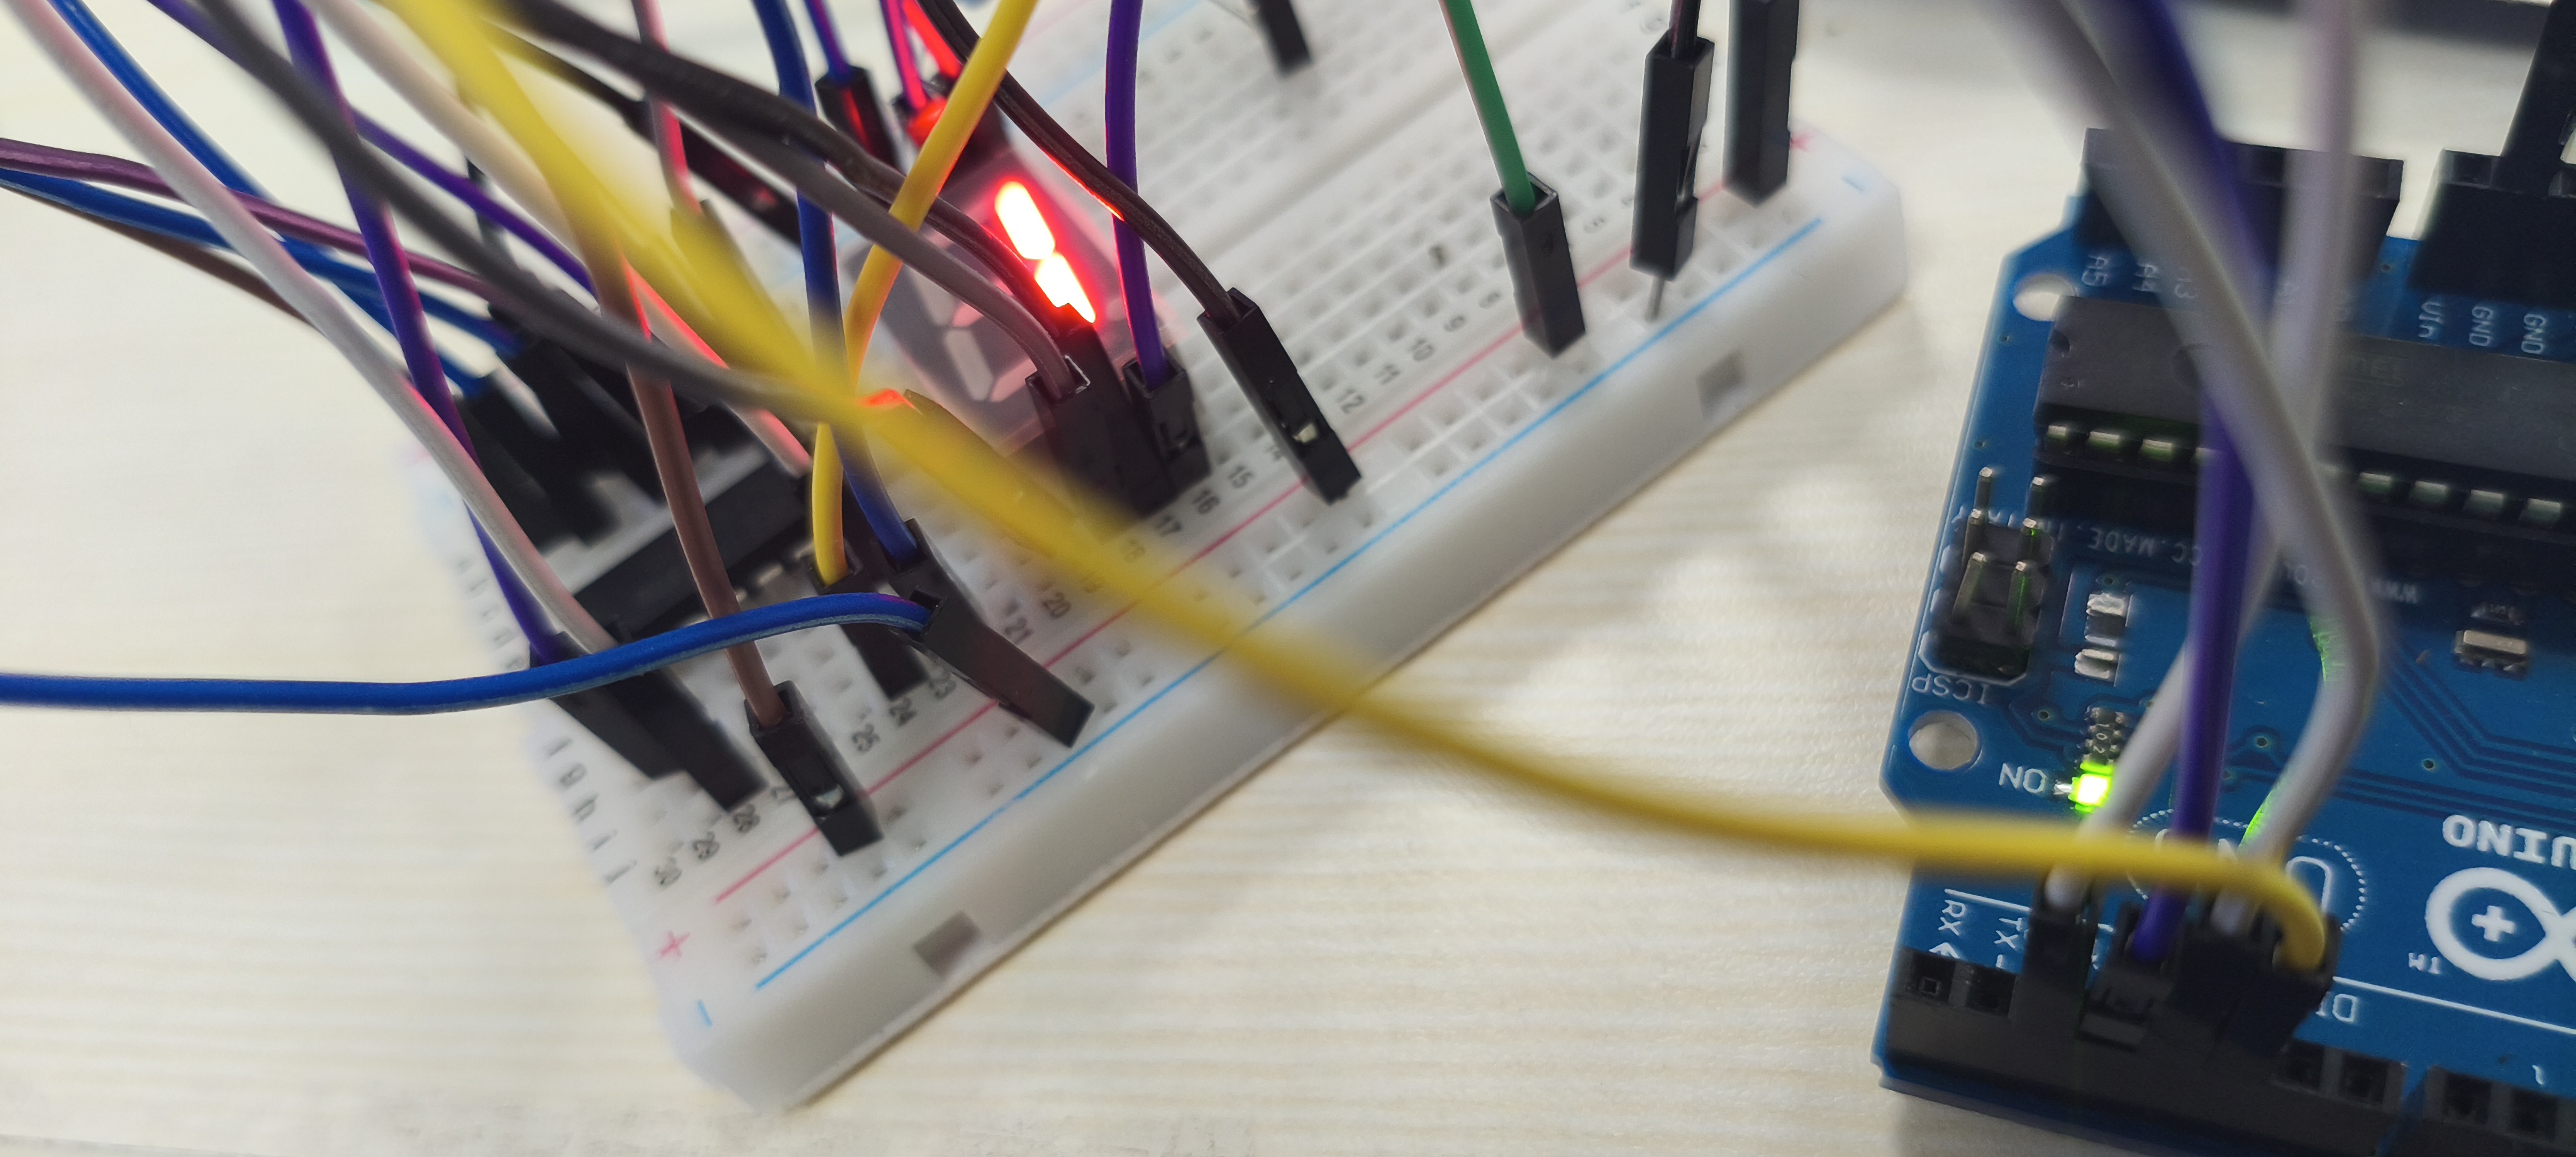
\includegraphics[width=0.45\textwidth]{output1.jpg}
\caption{Output Showing 1}
\end{figure}

\begin{figure}[H]
\centering
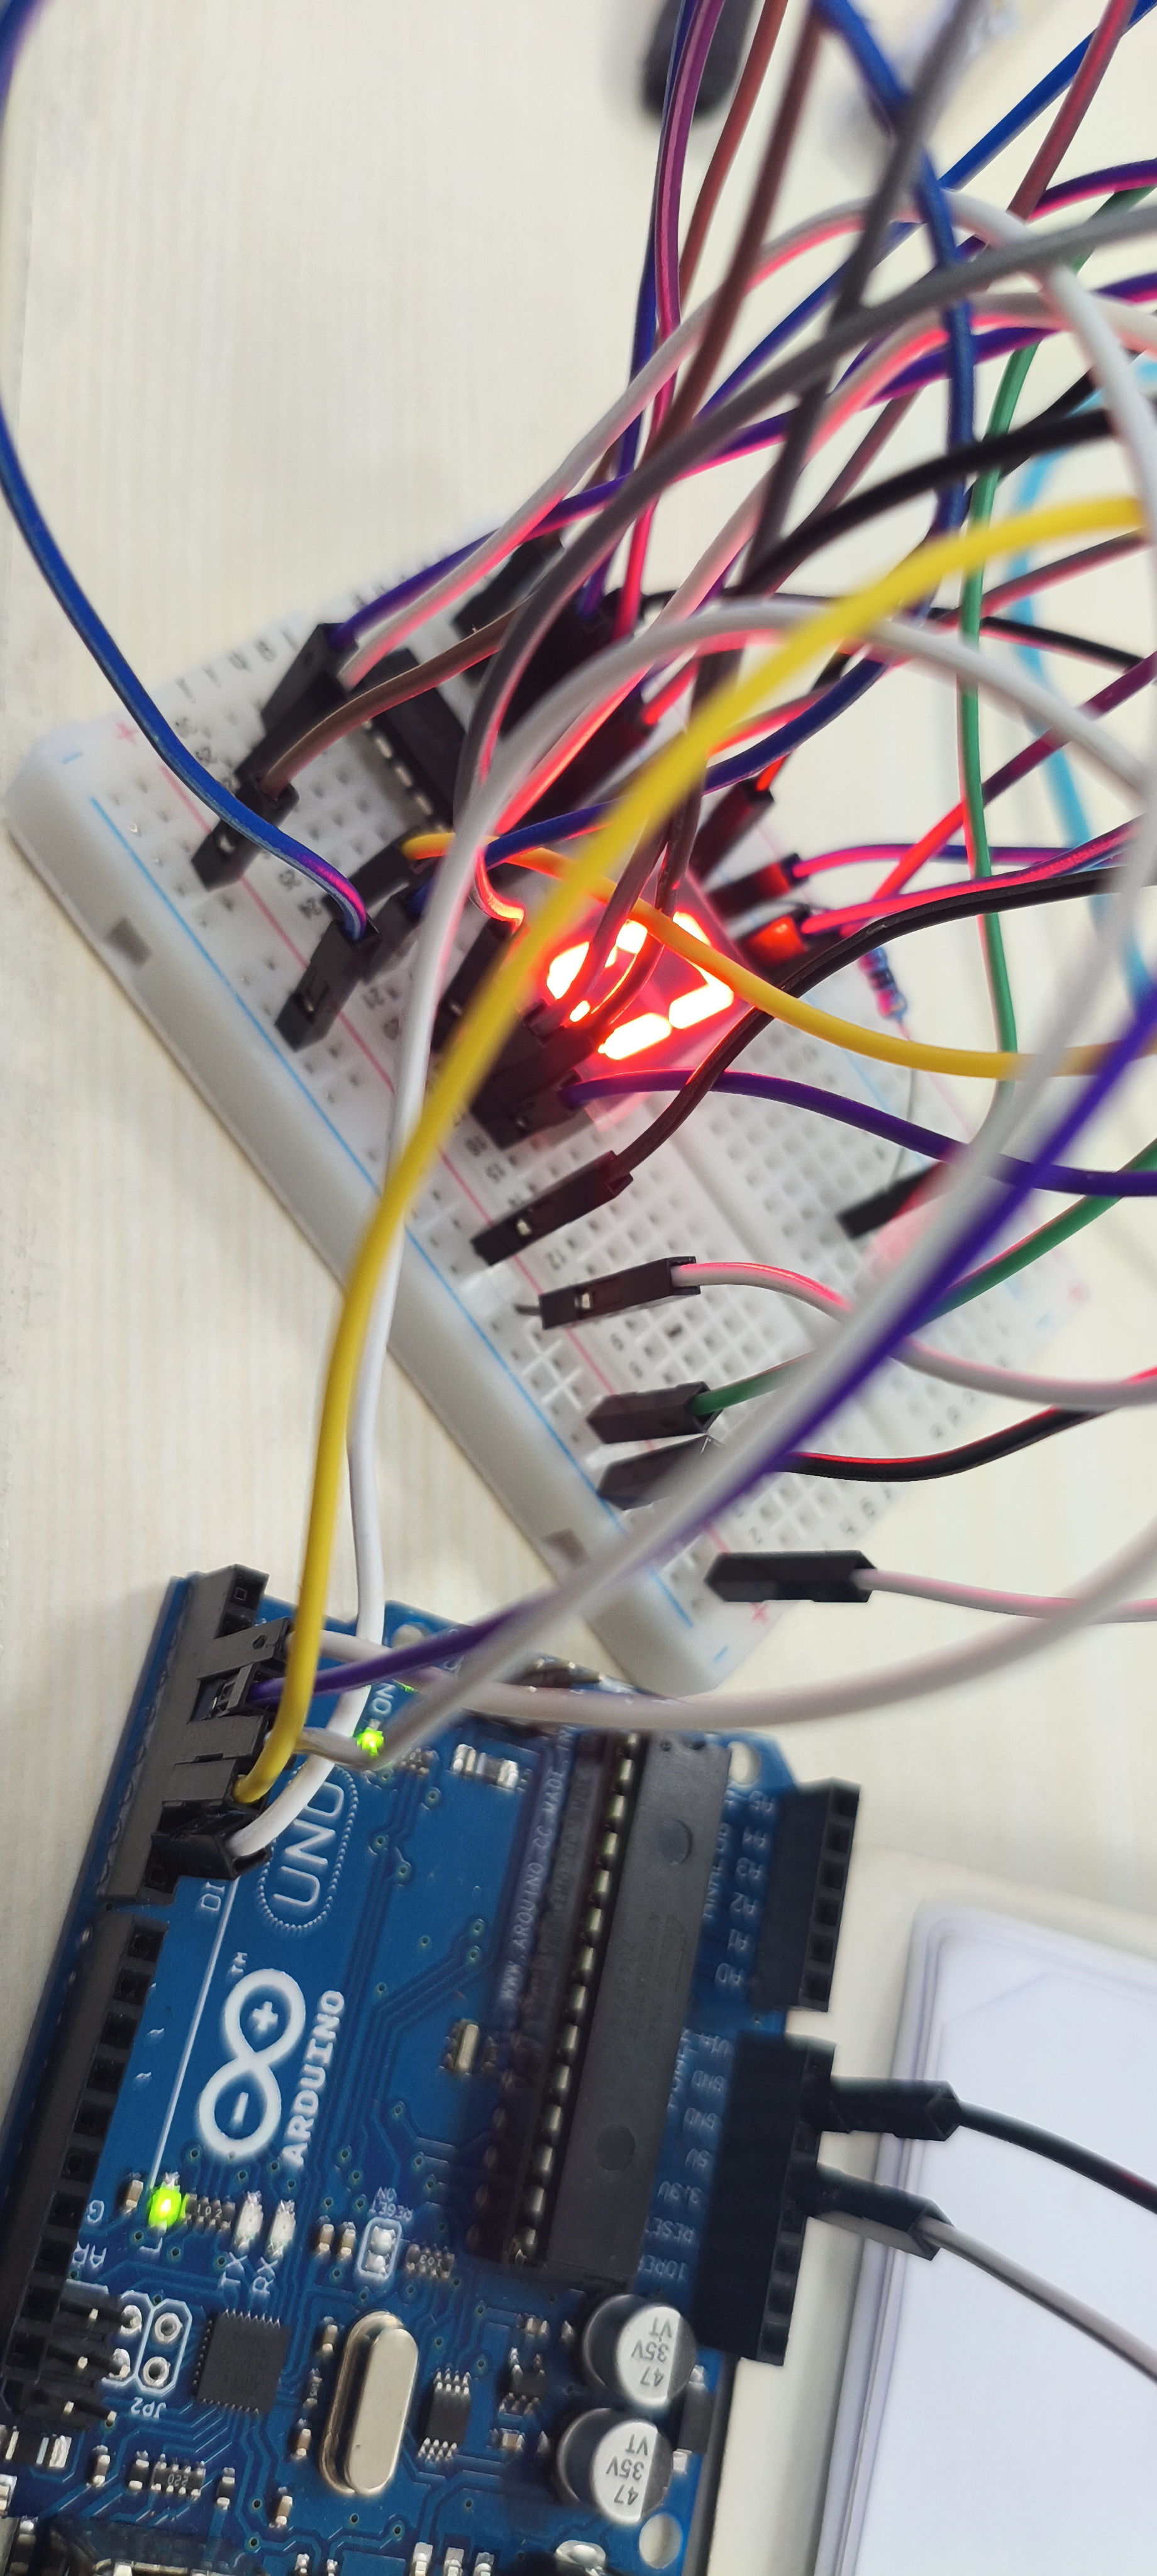
\includegraphics[width=0.45\textwidth]{output0.jpg}
\caption{Output Showing 0}
\end{figure}

\section{Result}

The Karnaugh Map expression was implemented using Arduino Uno and IC 7447.

[
A=\bar{W}\bar{Z}
]

For W=0 and Z=0,

[
A=1
]

Therefore the seven segment display shows 1.

\end{document}
